\documentclass[10pt,sigplan,screen,nonacm]{acmart}
\usepackage{subcaption}
\usepackage{tikz}
\usetikzlibrary{arrows.meta, positioning}

\setcopyright{none}

\begin{document}

\title{Evaluating and Improving the Security of AI-Based Code Assistants}
\subtitle{CS 329M Project Proposal}

\author{Timothy Gu}
\affiliation{%
  \institution{Stanford University}
  \city{Stanford}
  \state{CA}
  \country{USA}}
\email{timothygu@stanford.edu}

\renewcommand{\shorttitle}{CS 329M Project Proposal}
\renewcommand{\shortauthors}{Gu}

\begin{abstract}
    Since Open\-AI released the Codex system in 2021 \cite{Chen2021EvaluatingLL}, there has been a significant increase in interest into using large machine learning (ML) models as programming aids. The concurrent introduction of commercial products based on these models, such as GitHub Copilot and Amazon Code\-Whis\-per\-er, further made these tools available to ordinary software developers. However, since these models are often trained on a large volume of publicly available source code of inconsistent quality, the security of inferred code is hardly a guarantee. We seek to concretely improve the security and usability of AI-driven code recommendation platforms. We will first quantify the security and quality of a few of these systems over a range of potential inputs. We then propose the use of input preprocessing, output scanning, and rules-based output rewriting as techniques in an overall outcome improvement system.
\end{abstract}

\maketitle

\section{Background}

\subsection{Assistant Services}
The study will focus on \emph{AI-driven programming assistants.} Examples for such services include line autocomplete services like Kite\footnote{\url{https://www.kite.com/}}, GitHub Copilot\footnote{\url{https://github.com/features/copilot}} and/or its underlying model Open\-AI Codex, and Amazon Code\-Whis\-per\-er\footnote{\url{https://aws.amazon.com/codewhisperer/}}.

\subsection{Security Issues}

The security industry has a variety of categorization schemes for vulnerabilities. Out of the 2021 edition of OWASP Top 10 \cite{owasp-top10} -- categories that represent ``the most critical security risks to web applications'' according to industry practioners --
% As of 2021, the list\footnote{\url{https://owasp.org/www-project-top-ten/}} identifies the following broad categories:
% \begin{enumerate}
%     \item Broken Access Control
%     \item Cryptographic Failures
%     \item Injection
%     \item Insecure Design
%     \item Security Misconfiguration
%     \item Vulnerable and Outdated Components
%     \item Identification and Authentication Failures
%     \item Software and Data Integrity Failures
%     \item Security Logging and Monitoring Failures
%     \item Server-Side Request Forgery
% \end{enumerate}
many of them represent failures in the software design or system configuration, which are typically undertaken by human developers and are not the most applicable to this study. As such, we will narrow our focus on the following items:
\begin{enumerate}
    \setcounter{enumi}{1}
    \item \textbf{Cryptographic Failures:} Recommendations include old or broken ciphers or those that fell out of the general recommendations.
    % Examples: broken hash functions (MD5, SHA-1), weak ciphers (RC4, DES), insecure protocols (SSL, TLSv1.0/1.1), insecure cipher modes of operations (Electronic Codebook (ECB), Counter mode (CTR)).
    
    \item \textbf{Injection:} Recommendations include injection vulnerabilities, like SQL injection in server code and cross-site scripting (XSS) in HTML generators.
\end{enumerate}

\subsection{Prior Work}
Some previous work has looked into security of large language model code assistants. \Citeauthor{nyuuserstudy} \cite{nyuuserstudy} ran a medium-scale user study comparing the coding performance of assisted and unassisted student programmers, finding no significant impact on security. A Stanford lab conducted similar research, though thus far unpublished \cite{labstudy}. However, as far as I am aware, there is no work that look into systematically improving the security of code assistants.

\section{Methodology}

\subsection{Quantifying the Problem}
We will first attempt to quantify how (in)secure code generated by assistant services are. We will collect prompts from existing open-source web application projects (both code and comments), datasets (e.g., Open\-AI's Human\-Eval evaluation set\footnote{\url{https://github.com/openai/human-eval}}). Then, we will pass prompts to each service, and run several code vulnerability scanners on the generated output. We may also incorporate human review for logic bugs or misused cryptographic primitives.

Notably, Amazon Code\-Whis\-per\-er already includes a code security scanner. However, in my experience it does not catch all vulnerabilities, including an obvious SQL injection attack vector in Python. So we will only use it in conjunction with traditional rules-based scanners.

% \begin{figure}
%     \centering
%     \includegraphics[width=\columnwidth]{figs/codewhisperer-sql-scan.png}
%     \caption{Amazon CodeWhisperer fails to catch an obvious SQL injection attack vector.}
%     \label{fig:codewhisperer-sql-scan}
% \end{figure}

\subsection{Improving Outcome}

In order to improve the outcome of programming assistants, we propose investigating a few interlocking methods. These include both MP-specific strategies like Input Preprocessing as well as more traditional methods that also apply to human-written code. See \autoref{fig:outcome} for a summary of how these techniques work together.

\begin{figure} \centering \small
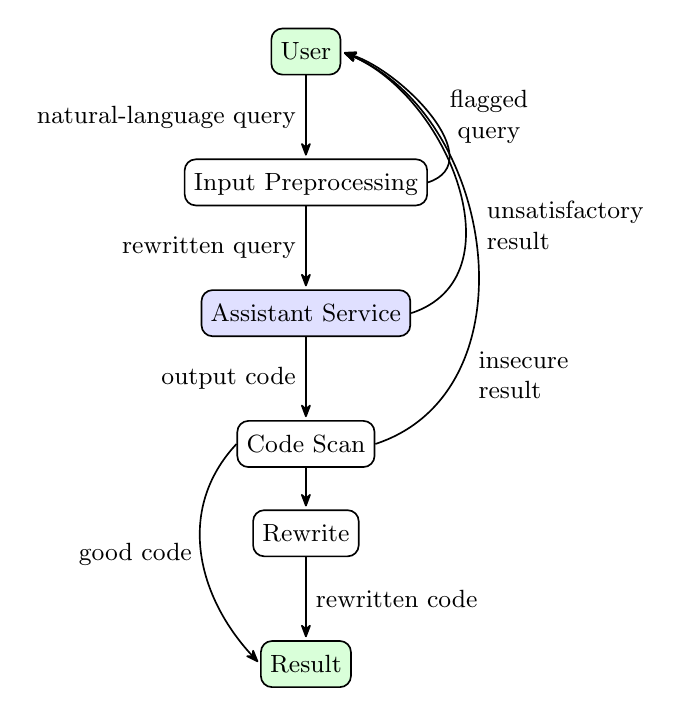
\begin{tikzpicture}[every node/.style={font={\small}}, >={Stealth[round,sep]}, semithick, yscale=0.9]
    \node[draw, rounded corners, text height=.8em, text depth=.2em, fill=green!15] (user) {User};
    \node[draw, rounded corners, text height=.8em, text depth=.2em] (input) [below=3em of user] {Input Preprocessing};
    \node[draw, rounded corners, text height=.8em, text depth=.2em, fill=blue!12] (assistant) [below=3em of input] {Assistant Service};
    \node[draw, rounded corners, text height=.8em, text depth=.2em] (scanning) [below=3em of assistant] {Code Scan};
    \node[draw, rounded corners, text height=.8em, text depth=.2em] (rewrite) [below=1.5em of scanning] {Rewrite};
    \node[draw, rounded corners, text height=.8em, text depth=.2em, fill=green!15] (result) [below=3em of rewrite] {Result};
    
    \draw[->] (user) to [edge node={node [left] {natural-language query}}] (input);
    \draw[->] (input) to [edge node={node [left] {rewritten query}}] (assistant);
    \draw[->] (assistant) to [edge node={node [left] {output code}}] (scanning);
    \draw[->] (scanning) -- (rewrite);
    \draw[->] (rewrite) to [edge node={node [right] {rewritten code}}] (result);
    \draw[->] (input.east) to [out=20, in=-20, edge node={node [right=0.3em, text width=1cm,align=center] {flagged query}}] (user.east);
    \draw[->] (assistant.east) to [out=20, in=-25, edge node={node [below right=0.3em, text width=2cm,align=left, xshift=0.5em] {unsatisfactory\\ result}}] (user.east);
    \draw[->] (scanning.east) to [out=20, in=-25, edge node={node [below right=0.3em, xshift=-0.5em, yshift=-3em, text width=2cm,align=left] {insecure\\ result}}] (user.east);
    \draw[->] (scanning.west) to [out=-130, in=130, edge node={node [left] {good code}}] (result.west);
\end{tikzpicture}
\caption{Overview of the outcome improvement engine.}
\label{fig:outcome}
\end{figure}

\subsubsection{Input Preprocessing}

AI-driven programming assistant models depend on a natural language prompt to generate relevant code. If the prompt describes an insecure software design, an assistant will likely generate insecure code. As an example, the prompt \emph{``Create a SQL query to find people with the given last name''} \balance invites SQL injection in the output code, since the best way to defeat SQL injection is by placing placeholders in the query and separating it from concrete values. We could flag badly designed prompts using natural language understanding, potentially using large language models themselves (see \autoref{fig:gpt-sql-check}).

\begin{figure}
    \centering
    \includegraphics[width=\columnwidth]{figs/gpt-sql-check2.png}
    \caption{Inquiring GPT-3 whether the given task requires returning a SQL query string}
    \label{fig:gpt-sql-check}
\end{figure}

Second, we could even investigate automatically rewriting the natural language input. One evaluation of Codex \cite{smitop} noticed that by default, Codex generated code with SQL injection vulnerability in response to \emph{``Insert \$name into the people table.''} However, after appending \emph{``safely''} to the prompt, Codex generated a SQL-based query free from injections.
Similarly, while the prompt \emph{``Generate user profile HTML for name''} elicited insecure code vulnerable to XSS, appending \emph{``using Jinja2''} made it safer by referencing a popular Python HTML template library.

\subsubsection{Output Scanning}

Despite our best attempts at flagging queries, it is likely impossible to completely avoid bad code from being generated. We can integrate industry-standard code scanners with IDE extensions to further flag suspicious output as a backstop mechanism. Code scanners such as Semgrep and Snyk as well as static analyzers like Coverity are widely adopted in industry. Emerging ML-based solutions such as Merly Mentor can also be integrated.

Though such tools often have high false positive rates, one may argue that model-written code requires a higher level of scrutiny compared to human-written code. Developers may also have higher tolerance for false positives, as the machine programmed code is new to them as well.

\subsubsection{Rules-based Output Rewriting}

A number of code scanning tools support automatic code rewriting for security (e.g., Snyk) and code style (code formatters and linters). We will attempt to create our own rewriter that detects injection vulnerabilities and ensure correct escaping is done.

\section{Timeline}

We propose the following timeline:

\begin{center}
    \begin{tabular}{@{}ll@{}} \toprule
        Time & Task \\ \midrule
        Week 3 & Submit project proposal \\
        Week 5 & Security evaluation \\
        Week 8 & Outcome improvement \\
        Week 9 & Project report due \\
        \bottomrule
    \end{tabular}
\end{center}

\bibliographystyle{ACM-Reference-Format}
\bibliography{project}

\end{document}
